\documentclass{article}

\newcommand{\doctitle}{compcoll 文本对比校对软件使用说明}
\newcommand{\docauthor}{v 1.02}
\newcommand{\dockeywords}{{diff}{compare}}
\newcommand{\docsubject}{}

\newcommand\mymainfont{DejaVu Serif}%{Times New Roman} %{DejaVu Serif}
\newcommand\mymonofont{DejaVu Sans Mono}%{FreeMono} %{WenQuanYi Micro Hei Mono} %{Monaco}
\newcommand\myboldfont{WenQuanYi Micro Hei Mono}%{AR PL UKai CN}%{YaHei Consolas Hybrid}%{黑体}%{標楷體}
\newcommand\mysansfont{DejaVu Sans}%{FreeSans}
\newcommand\myitalicfont{DejaVu Serif}%{Times New Roman} %{Garamond}

\newcommand\mycjkboldfont{WenQuanYi Micro Hei Mono}%{Adobe Heiti Std}%{AR PL UKai CN}%{YaHei Consolas Hybrid}%{黑体}%{標楷體}
\newcommand\mycjkitalicfont{Adobe Kaiti Std}
\newcommand\mycjkmainfont{AR PL UMing CN}%{Adobe Song Std}%{仿宋}%{宋体}%{新宋体}%{文鼎PL新宋}%
\newcommand\mycjksansfont{Adobe Ming Std}
\newcommand\mycjkmonofont{WenQuanYi Micro Hei Mono}%{AR PL UMing CN}%{WenQuanYi Micro Hei Mono}

\usepackage{ifthen}
\usepackage{ifpdf}
\usepackage{ifxetex}
\usepackage{ifluatex}

\usepackage{color}
\usepackage[rgb]{xcolor}

\usepackage{url}
\usepackage{array}

\usepackage{courier}
\usepackage{listings} % list the source code
\definecolor{ForestGreen}{rgb}{0.13,0.55,0.13}

\lstset{
    language=C,
    captionpos=b, %t,
    tabsize=3,
    basicstyle=\footnotesize\ttfamily, %basicstyle=\ttfamily\normalsize, %basicstyle=\small\ttfamily, %\normalfont\ttfamily, % \large\ttfamily, % \small\ttfamily, % \footnotesize\ttfamily, % \scriptsize\ttfamily, % Standardschrift,
    numbers=left,               %左侧显示行号 往左靠,还可以为right,或none,即不加行号
    stepnumber=1,               %若设置为2,则显示行号为1,3,5,即stepnumber为公差,默认stepnumber=1
    %numberstyle=\tiny,         %行号字体用小号
    numberstyle={\color[RGB]{0,192,192}\tiny} ,%设置行号的大小,大小有tiny,scriptsize,footnotesize,small,normalsize,large等
    numbersep=8pt,              %设置行号与代码的距离,默认是5pt
    breaklines=true,            %对过长的代码自动换行
    showstringspaces=false,     %不显示代码字符串中间的空格标记
    frame=shadowbox, %=lines,                    %把代码用带有阴影的框圈起来
    stringstyle=\ttfamily,      % 代码字符串的特殊格式
    commentstyle=\color{ForestGreen}, %\color{red!50!green!50!blue!50}, %浅灰色的注释
    rulesepcolor=\color{red!20!green!20!blue!20}, %代码块边框为淡青色
    keywordstyle=\color{blue!90}\bfseries,        %代码关键字的颜色为蓝色,粗体
    backgroundcolor=\color[rgb]{1,1,1},%\color[RGB]{245,245,244},   %代码背景色 \color[rgb]{0.91,0.91,0.91}
    framextopmargin=2pt,framexbottommargin=2pt,abovecaptionskip=-3pt,belowcaptionskip=3pt,
%    xleftmargin=4em,xrightmargin=4em, % 设定listing左右的空白
%    %language={[ISO]C++},       %language为,还有{[Visual]C++}
%    alsolanguage=Java,
%    %alsolanguage=[ANSI]C,      %可以添加很多个alsolanguage,如alsolanguage=matlab,alsolanguage=VHDL等
%    %alsolanguage= tcl,
%    alsolanguage= XML,
%    keepspaces=true,            %
%    breakindent=22pt,           %
%    breakindent=4em,            %
%    showspaces=false,           %
%    flexiblecolumns=true,       %
%    breakautoindent=true,       %
%    aboveskip=1em,              %代码块边框
%    %% added by http://bbs.ctex.org/viewthread.php?tid=53451
%    fontadjust,
%    texcl=true,
%    escapeinside=``,            %在``里显示中文
%    %escapebegin=\begin{CJK*}{GBK}{hei},escapeend=\end{CJK*},
%    % 设定中文冲突,断行,列模式,数学环境输入,listing数字的样式
%    extendedchars=false,columns=flexible,
%    mathescape=false,
%    % numbersep=-1em,
    emph={label}
}

\renewcommand{\ttdefault}{pcr}

\definecolor{darkgreen}{cmyk}{0.7, 0, 1, 0.5}
\definecolor{darkblue}{rgb}{0.1, 0.1, 0.5}
\lstdefinelanguage{diff}
{
    keywords={+, -, \ , @@, diff, index, new},
    sensitive=false,
    morecomment=[l][""]{\ },
    morecomment=[l][\color{darkgreen}]{+},
    morecomment=[l][\color{red}]{-},
    morecomment=[l][\color{darkblue}]{@@},
    morecomment=[l][\color{darkblue}]{diff},
    morecomment=[l][\color{darkblue}]{index},
    morecomment=[l][\color{darkblue}]{new},
    morecomment=[l][\color{darkblue}]{similarity},
    morecomment=[l][\color{darkblue}]{rename},
}

\lstdefinelanguage{JavaScript}{
  keywords={typeof, new, true, false, catch, function, return, null, catch, switch, var, if, in, while, do, else, case, break},
  keywordstyle=\color{blue}\bfseries,
  ndkeywords={class, export, boolean, throw, implements, import, this},
  ndkeywordstyle=\color{darkgray}\bfseries,
  identifierstyle=\color{black},
  sensitive=false,
  comment=[l]{//},
  morecomment=[s]{/*}{*/},
  %commentstyle=\color{purple}\ttfamily,
  commentstyle=\color{green}\ttfamily,
  stringstyle=\color{red}\ttfamily,
  morestring=[b]',
  morestring=[b]"
}


%\usepackage[adobefonts]{ctex} %nofonts,adobefonts
\usepackage[nofonts]{ctex} %nofonts,adobefonts
%\usepackage[fallback]{xeCJK}

%\usepackage{CJKfntef}

\setCJKmainfont[BoldFont=\mycjkboldfont, ItalicFont=\mycjkitalicfont]{\mycjkmainfont}
\setCJKsansfont{\mycjksansfont}

%\setCJKmainfont[BoldFont=\mycjkboldfont, ItalicFont=\mycjkitalicfont]{\mycjkmainfont}
%\setCJKsansfont{\mycjksansfont}%{Adobe Ming Std} %{AR PL UMing CN} %{Microsoft YaHei}
%\setCJKmonofont{\mycjkmonofont}
%
%\setmonofont[Scale=0.8]{\mymonofont} % 英文等宽字体
%\setsansfont{\mysansfont}       % 英文无衬线字体 %\setmainfont{\mymainfont}        % 英文衬线字体, setmainfont=setromanfont
%\setromanfont[Mapping=tex-text,  % 沿用 LaTex 的一些习惯的标点转换,例如 en-dash 以两个减号表示
%    Ligatures={Required,Common}, % 如果此字体内置 Ligatures 定义则启用
%    ItalicFont={\myitalicfont},  % 斜体用 Times Italic,严格来说只有拉丁子母有斜体。
%    BoldFont={\myboldfont}]      % 粗体用字体
%    {\mymainfont}                % 内文使用字体, Linux 下用 "fc-list :lang=zh-cn" 列出支持的中文字体
%} % \usefontspeczh


%\setCJKmainfont{SimSun}
%\setCJKfallbackfamilyfont{rm}{SimSun-ExtB}

%\newcommand\myfontdir{fonts/}

%\setCJKmainfont[Path=\myfontdir,
    %FallBack={khangxidict-1.023-full.otf},%{SourceHanSans-Light.otf},
    %BoldFont={AdobeHeitiStd-Regular.otf},
    %ItalicFont={AdobeKaitiStd-Regular.otf},
    %ItalicFeatures={RawFeature={slant=0.17}}, % 定义 \itshape 为斜体
    %BoldItalicFeatures={RawFeature={slant=0.17}}, % 定义 \bfseries\itshape 为斜体
    %AutoFakeBold,AutoFakeSlant]{fzqkbyss-1.00.ttf} % fzqkbyss is 方正清刻体简体 GB2312

%\setCJKfallbackfamilyfont{\CJKrmdefault}[AutoFakeSlant]{
    %[Path=\myfontdir]{khangxidict-1.023-full.otf},
    %[Path=\myfontdir]{mingliub-7.01.ttc},
    %[Path=\myfontdir]{SourceHanSans-Light.otf},
%}


% ============================================
% Check for PDFLaTeX/LaTeX
% ============================================
\newcommand{\outengine}{xetex}
\newif\ifpdf
\ifx\pdfoutput\undefined
  \pdffalse % we are not running PDFLaTeX
  \ifxetex
    \renewcommand{\outengine}{xetex}
  \else
    \renewcommand{\outengine}{dvipdfmx}
  \fi
\else
  \pdfoutput=1 % we are running PDFLaTeX
  \pdftrue
  \usepackage{thumbpdf}
  \renewcommand{\outengine}{pdftex}
  \pdfcompresslevel=9
\fi
\usepackage[\outengine,
    bookmarksnumbered, %dvipdfmx
    %% unicode, %% 不能有unicode选项,否则bookmark会是乱码
    colorlinks=true,
    citecolor=red,
    urlcolor=blue,        % \href{...}{...} external (URL)
    filecolor=red,      % \href{...} local file
    linkcolor=black, % \ref{...} and \pageref{...}
    breaklinks,
    pdftitle={\doctitle},
    pdfauthor={\docauthor},
    pdfsubject={\docsubject},
    pdfkeywords={\dockeywords},
    pdfproducer={Latex with hyperref},
    pdfcreator={pdflatex},
    %%pdfadjustspacing=1,
    pdfborder=1,
    pdfpagemode=UseNone,
    pagebackref,
    bookmarksopen=true]{hyperref}

% --------------------------------------------
% Load graphicx package with pdf if needed 
% --------------------------------------------
\ifxetex    % xelatex
    \usepackage{graphicx}
\else
    \ifpdf
        \usepackage[pdftex]{graphicx}
        \pdfcompresslevel=9
    \else
        \usepackage{graphicx} % \usepackage[dvipdfm]{graphicx}
    \fi
\fi

%% \DeclareGraphicsRule{.jpg}{eps}{.bb}{}
%% \DeclareGraphicsRule{.png}{eps}{.bb}{}
\graphicspath{{./} {figures/}}
\usepackage{flafter} % 防止图形在文字前


%\usepackage[margin=1.8cm,nohead]{geometry}
\usepackage[margin=1in,nohead]{geometry}
%\usepackage[top=1in,bottom=1in,left=1.25in,right=1.25in]{geometry} % 设置页边距
%\setlength{\belowcaptionskip}{1em} % 设置caption之后的距离


\title{\doctitle}
\author{\docauthor}
\date{}

\begin{document}
\maketitle



\section{简介}


\texttt{compcoll} 是一套用于对比两个相近文本的工具。该工具可用于通过比较同一个内容的两个不同出处的文本的校对。

本软件是文字级别的文本对比,
相对于其他软件,例如:

diff, git diff --word-diff, svn diff 等工具是基于行比较的。对于每行都是一整段的文本,如果其中有大量的不同,不能区分其中的每个相异之处;
而且,如果所比较的两个文本内容大致相同,但分行分段不同时,这些 diff 工具就区分不出来了。

cmp 工具是可以比较出两段文本第一个不同之处。但如果要找出所有不同,则需要另外自行实现复杂脚本,而且很难实现文本的最小差异的识别。

本软件可以找出两个文本之间最小差异之处,并输出比较结果。


\subsection{特性}

\begin{itemize}
  \item 找出两个文本间,字符级别的最小不同之处。
  \item 可通过章回处理任意大小的文本。
  \item 自动识别输入文本的编码,用户可以专注于文件内容而不必处理繁琐的编码转换。如输入格式可以是 Big5, GB18030 等编码。
  \item 通过 html 格式输出结果;可使用任意浏览器查看结果,可以通过 CSS 用户定制输出式样。
  \item 采用\texttt{bash}脚本来整合核心功能,达到最大的灵活性和良好的移植特性。支持批处理和人工介入处理。
\end{itemize}


\subsection{限制}

\begin{itemize}
  \item 输入文件只能是文本类格式,如 HTML、TXT 等。WORD 格式的文件可以通过 OFFICE 输出成 HTML 或者 TEXT 格式后再通过本软件处理。
  \item 软件对比的目的是找出文本间不同的字,因而最小单位是字符,包括中文字符和英文字符,所以不支持外文,如英文,的单词级别的变形对比。
  \item 虽使用了最优算法,但软件仍受其理论上限所影响。为最大化性能,建议所对比的单个文件中的字符数(中文字符和英文字符)不超过内存大小的开方。(这个限制只是内部对每章回字数的限制;即软件可针对任意超过100万字大小的文本通过章节拆分文本,使每章都在单独的一个文件中,而这里指的是这个每章中的字符数。)
例如,在1GB($10^9$)内存的机器上,其单个文件字符数最大上限大概是32000个字符。
\end{itemize}


\section{Windows 下安装说明}

本软件支持Windows,已经在 Windows XP 和 Windows 7 中测试通过。
安装分两部分,一个是基本\texttt{bash}环境的安装和本软件包的安装。

\begin{itemize}
  \item \texttt{bash}环境:这个是为了后面脚本的灵活处理而设置的。我们这里采用开源项目中附带的 bash 环境。
  \item 本软件包:是一些功能脚本和支持软件的集成。只需要将运行脚本包解压到一个目录下,根据需求修改参数,直接执行即可,不用安装。
  \item 文本编辑器: 选装,因 Windows 自带的编辑器太弱,还有可能破坏文件。
\end{itemize}



\subsection{\texttt{bash}环境}

我们选择了同时有版本控制管理功能和\texttt{bash}环境的软件包 \href{https://code.google.com/p/gitextensions/}{Git Extensions},
一方面其方便地安装设置了我们所用的\texttt{bash}环境,另外,GIT还是一个很好的分布式版本控制软件,
可以用于我们文本的版本管理。

下载地点: \url{https://code.google.com/p/gitextensions/downloads/list}

请选择完全版本,如 \href{https://code.google.com/p/gitextensions/downloads/detail?name=GitExtensions24703SetupComplete.msi&can=2&q=}{GitExtensions24703SetupComplete.msi}

下载后,可用鼠标双击即可开始安装。


要注意的是,该软件需要 Microsoft .NET Framework 4 支持,如果没有预安装的话,需要从微软主页上下载。
Microsoft .NET Framework 4 Web 安装程序 分 
\href{http://www.microsoft.com/zh-cn/download/details.aspx?id=22833}{.NET Framework 4(独立安装程序)}
和
\href{http://www.microsoft.com/zh-CN/download/details.aspx?id=17851}{Microsoft .NET Framework 4(Web 安装程序)}
两种,独立安装程序只要下一次就可以安装,而 Web安装程序 则需要联网安装;如果独立安装程序安装不成功的话,可以试下Web 安装程序。



\begin{figure}[ht]\centering
  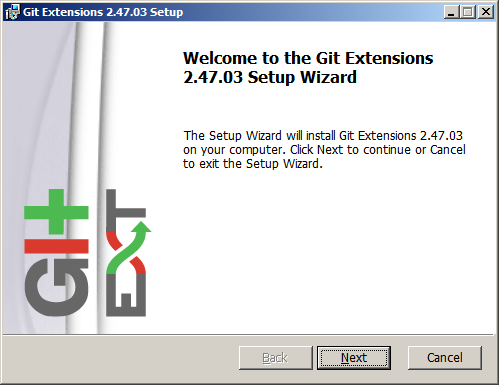
\includegraphics[width=0.45\textwidth]{figures/git/set1.png}
  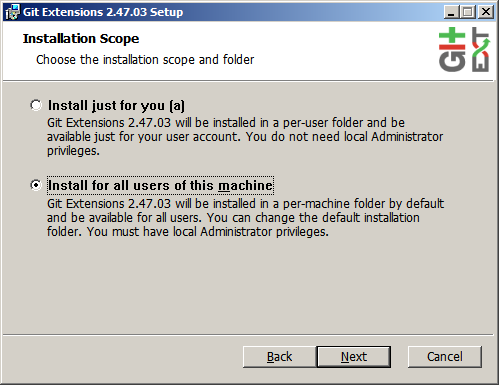
\includegraphics[width=0.45\textwidth]{figures/git/set2.png}
  \caption{开始安装,鼠标点击 ``Next'' 按钮。}\label{fig:set1}
\end{figure}


其中在图 \ref{fig:set3} 中显示时,记得要另外勾选 ``MsysGit'',因为该选项缺省是不安装的。

\begin{figure}[ht]\centering
  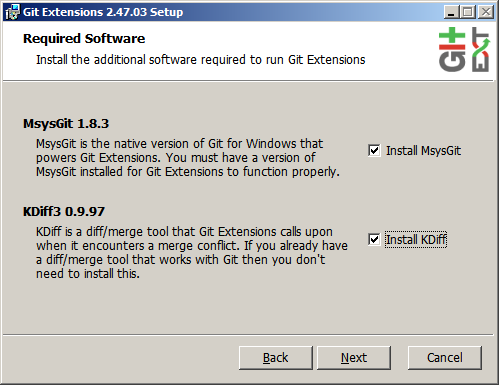
\includegraphics[width=0.45\textwidth]{figures/git/set3.png}
  \caption{选择bash环境。\textcolor{red}{注意要勾选 ``MsysGit''} ! 选择后,鼠标点击 ``Next'' 按钮。}\label{fig:set3}
\end{figure}


\begin{figure}[ht]\centering
  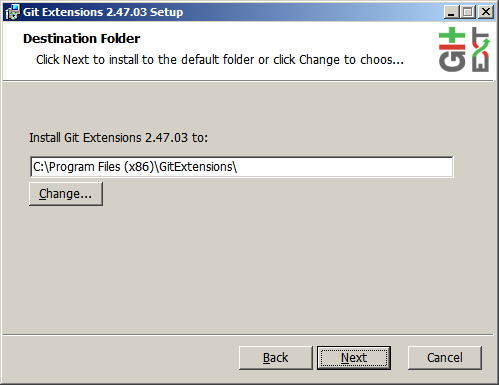
\includegraphics[width=0.45\textwidth]{figures/git/set4.png}
  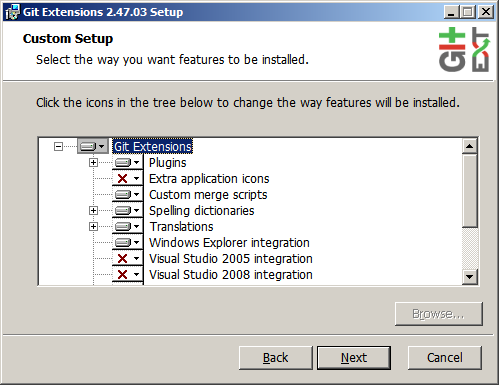
\includegraphics[width=0.45\textwidth]{figures/git/set5.png}
  \caption{鼠标点击 ``Next'' 按钮。}\label{fig:set4}
\end{figure}


\begin{figure}[ht]\centering
  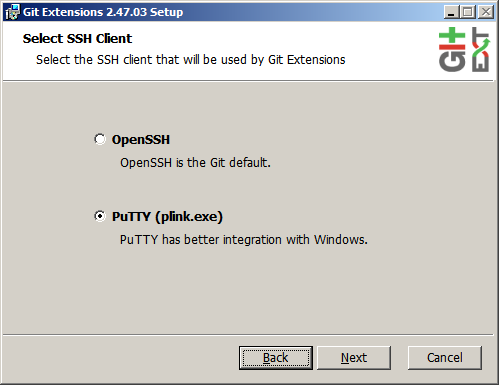
\includegraphics[width=0.45\textwidth]{figures/git/set6.png}
  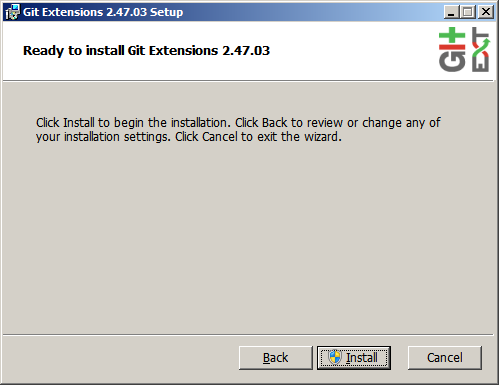
\includegraphics[width=0.45\textwidth]{figures/git/set7.png}
  \caption{鼠标先后点击 ``Next'' 和 ``Install'' 按钮。}\label{fig:set6}
\end{figure}


\begin{figure}[ht]\centering
  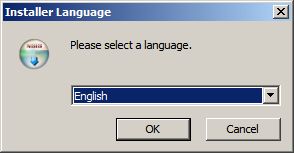
\includegraphics[width=0.45\textwidth]{figures/git/set8-1.png}
  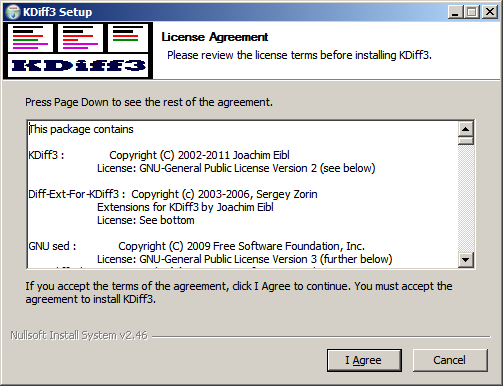
\includegraphics[width=0.45\textwidth]{figures/git/set8-2.png}
  \caption{安装 KDiff3,鼠标先后点击 ``OK'' 和 ``I Agree'' 按钮。}\label{fig:set8-1}
\end{figure}

\begin{figure}[ht]\centering
  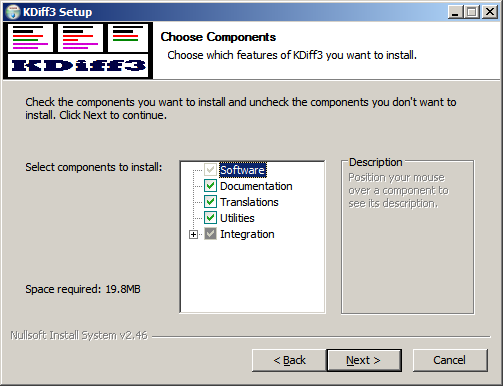
\includegraphics[width=0.45\textwidth]{figures/git/set8-3.png}
  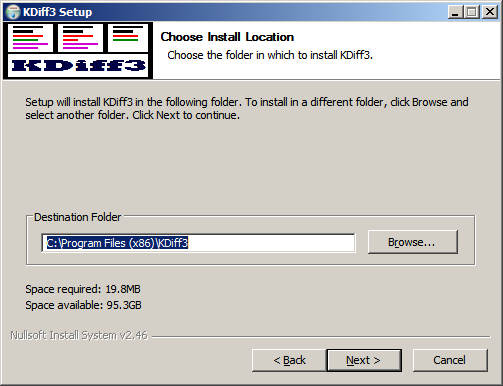
\includegraphics[width=0.45\textwidth]{figures/git/set8-4.png}
  \caption{鼠标点击 ``Next'' 按钮。}\label{fig:set8-3}
\end{figure}

\begin{figure}[ht]\centering
  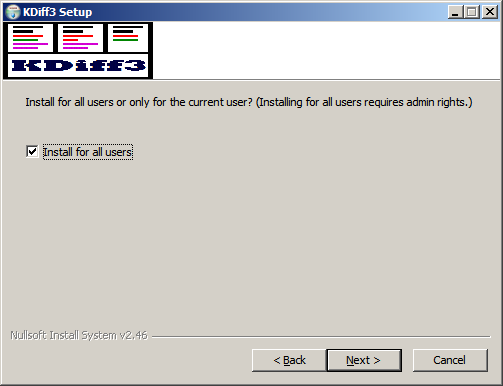
\includegraphics[width=0.45\textwidth]{figures/git/set8-5.png}
  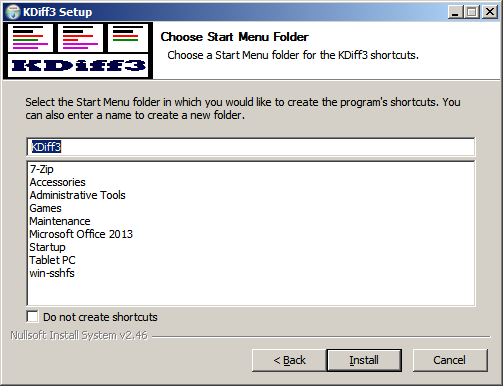
\includegraphics[width=0.45\textwidth]{figures/git/set8-6.png}
  \caption{鼠标点击 ``Next'' 按钮。}\label{fig:set8-5}
\end{figure}

\begin{figure}[ht]\centering
  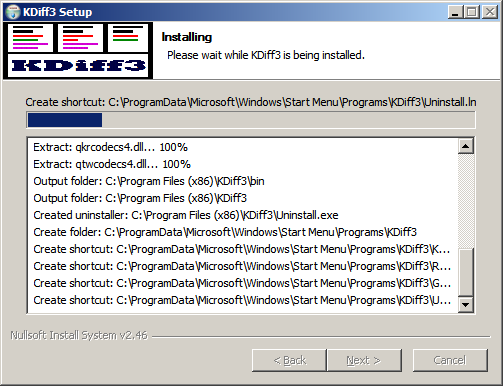
\includegraphics[width=0.45\textwidth]{figures/git/set8-7.png}
  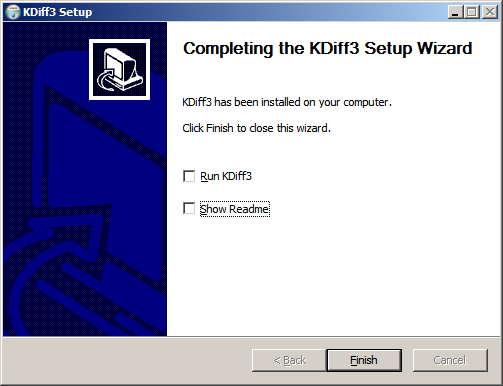
\includegraphics[width=0.45\textwidth]{figures/git/set8-8.png}
  \caption{鼠标点击 ``Finish'' 按钮。}\label{fig:set8-7}
\end{figure}



\begin{figure}[ht]\centering
  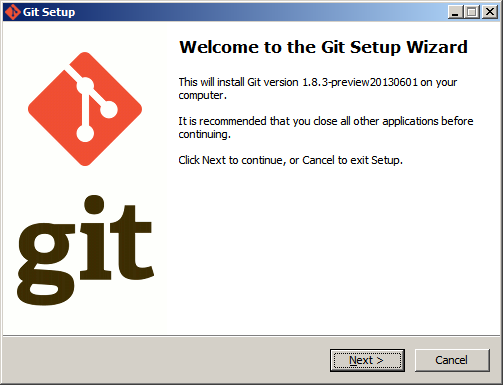
\includegraphics[width=0.45\textwidth]{figures/git/set9-1.png}
  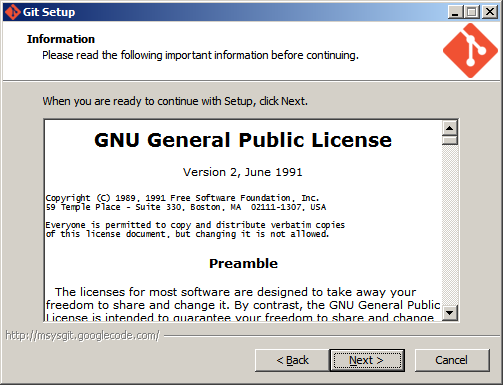
\includegraphics[width=0.45\textwidth]{figures/git/set9-2.png}
  \caption{安装和设置 Git,鼠标点击 ``Next'' 按钮。}\label{fig:set9-1}
\end{figure}

\begin{figure}[ht]\centering
  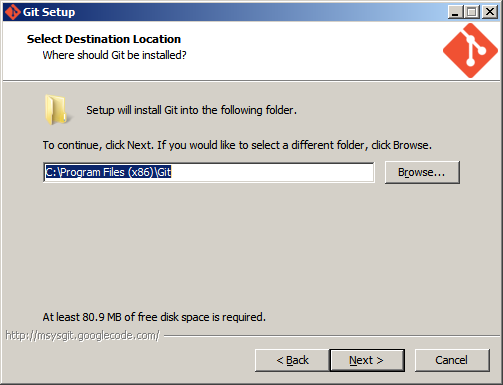
\includegraphics[width=0.45\textwidth]{figures/git/set9-3.png}
  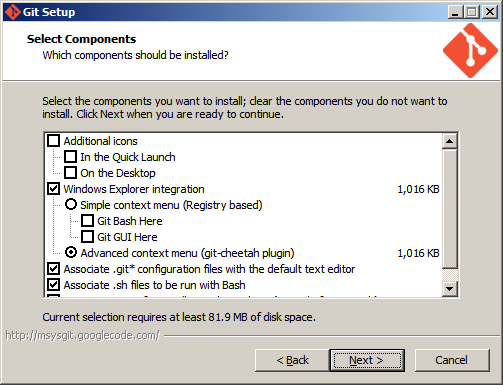
\includegraphics[width=0.45\textwidth]{figures/git/set9-4.png}
  \caption{鼠标点击 ``Next'' 按钮。}\label{fig:set9-3}
\end{figure}


然后在图\ref{fig:set9-5}中显示的选择 Git bash 时,
选择可在全局运行bash命令的 ``Run Git and included Unix tools from the Windows Command Prompt''。

\begin{figure}[ht]\centering
  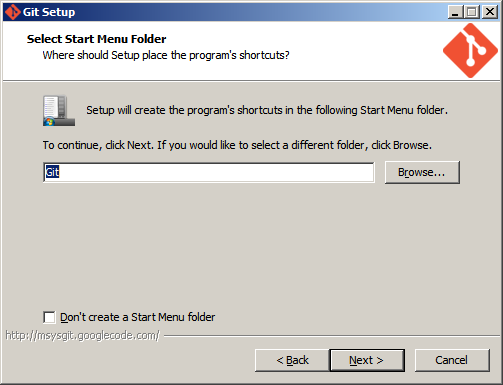
\includegraphics[width=0.45\textwidth]{figures/git/set9-5.png}
  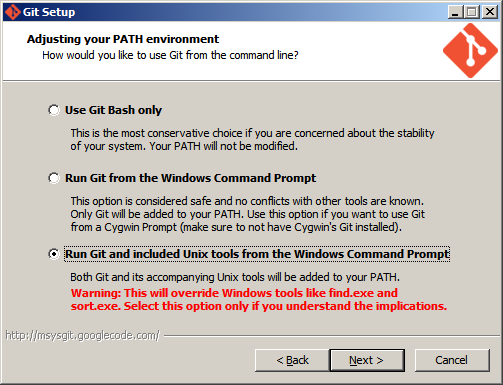
\includegraphics[width=0.45\textwidth]{figures/git/set9-6.png}
  \caption{\textcolor{red}{这步很重要,需要选择 ``Run Git and included Unix tools from the Windows Command Prompt''},然后鼠标点击 ``Next'' 按钮。}\label{fig:set9-5}
\end{figure}



\begin{figure}[ht]\centering
  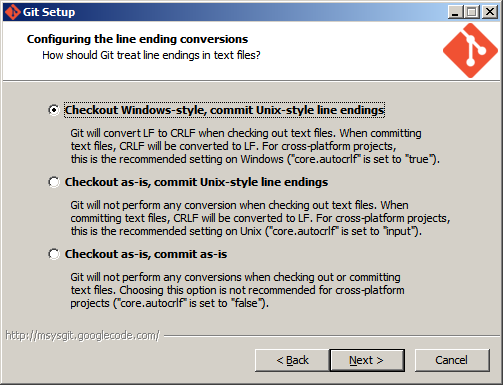
\includegraphics[width=0.45\textwidth]{figures/git/set9-7.png}
  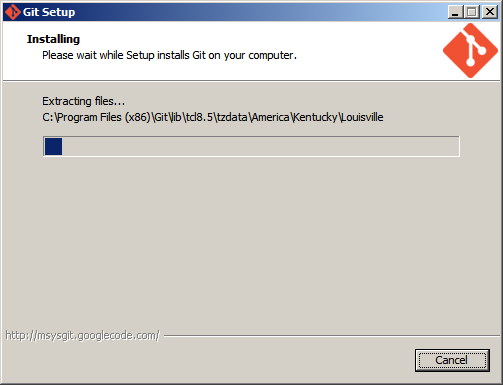
\includegraphics[width=0.45\textwidth]{figures/git/set9-8.png}
  \caption{鼠标点击 ``Next'' 按钮。}\label{fig:set9-7}
\end{figure}

\begin{figure}[ht]\centering
  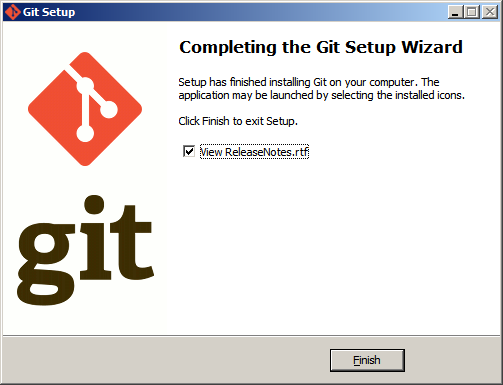
\includegraphics[width=0.45\textwidth]{figures/git/set9-9.png}
  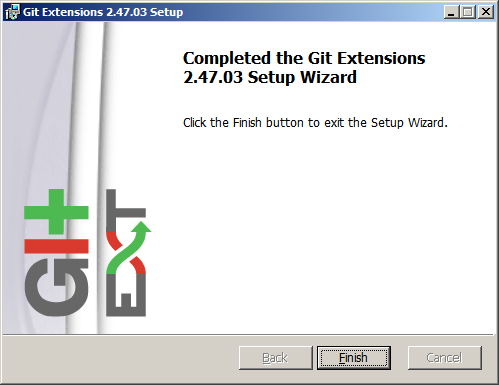
\includegraphics[width=0.45\textwidth]{figures/git/set10.png}
  \caption{安装完成Git}\label{fig:set9-9}
\end{figure}


\subsection{开源文本编辑器} \label{chap:madeditinstall}
Windows 自带的编辑器可能会破坏脚本内容,所以在需要修改定制软件时,
推荐使用开源软件 \href{http://code.google.com/p/madedit-pv/}{MadEdit},

同时,该软件还支持繁中转换,文件编码自动识别等强大功能。

可以在这里下载:

\url{http://code.google.com/p/madedit-pv/downloads/list}

毋须安装,解压即可使用!



\cleardoublepage



\subsection{compcoll 及快速入门}

将本安装包解压到一个目录下,可以看到一些以后缀名 \texttt{.sh} 结束的脚本文件。
其中 \texttt{run1.sh} 和 \texttt{run2.sh} 是测试用的两个脚本,分别用于拆分章节和对比章节。
这两个脚本很简单,只有一两行,你只需要修改这两个脚本中的目录名参数,来用于自己的项目。其他工作都是自动进行的。

如下是几个测试用的目录介绍。这些目录用于你安装完成后,测试安装是否成功用的。
\begin{itemize}
  \item \texttt{jpmch-02-ft-htm}: 需要对比的文本原始文件,编码为 GB18030 的繁体。
  \item \texttt{jpmch-03-ft-htm}: 需要对比的另一个文本原始文件,编码为 BIG5 的繁体。
  \item \texttt{jpmch-02-ft-txtout}: 经过脚本 \texttt{run1.sh} 生成的中间文本文件,使用单个文件分割各个章节,编码为 UTF-8, 为对比做准备。
  \item \texttt{jpmch-03-ft-txtout}: 同上。
  \item \texttt{cmp-jpmch-02-ft-vs-03}: 经过脚本 \texttt{run2.sh} 生成的对比文本HTML文件。比较了目录 \texttt{jpmch-02-ft-txtout} 和 \texttt{jpmch-03-ft-txtout} 中各个顺序文件。
\end{itemize}

你可以将这些目录先挪一个安全的地方,然后复制一份目录 \texttt{jpmch-02-ft-htm} 和 \texttt{jpmch-03-ft-htm}
出来到脚本目录(\texttt{run1.sh} 和 \texttt{run2.sh}等)下。然后\emph{双击鼠标运行} \texttt{run1.sh} 就会生成目录 \texttt{jpmch-02-ft-txtout} 和 \texttt{jpmch-03-ft-txtout}。

接着按照章节 \ref{chap:splitdata} 中介绍的方法稍做整理,再\emph{双击鼠标运行脚本} \texttt{run2.sh} 生成最终的对比文本目录  \texttt{cmp-jpmch-02-ft-vs-03}。你可以用这些你机器上生成的文件比较软件包所附带的文件,如果相同则表示安装成功。



\section{使用说明}

软件中的优化算法要求所比较的文本长度有限,所以需要预处理原始文本。
要求从两个数据源而来的处理后的两个子文本是一一对应的内容,如某一章节的内容;或者如果章节太长的话,还要进一步分块而且使其一一对应。

本软件包中已经提供了对于以章节来分块的拆分章节便利工具,这是通过扫描文本中是否含有 ``第xx回'' 来判定各个章回的起始位置。
这个工具主要是方便用户切分各章,以免手动处理上百章以上的文档。
如果各章节不是以这个开头,则需要另外修改分块脚本,或者手工处理。


之后的对比章节主程序需要输入文件的编码为UTF-8格式。
对于经过拆分章节工具处理的输出文件就可以直接用于对比章节。
对于用户自己手工处理过的分段数据文件,也请使用拆分章节工具处理一下(如修改并双击鼠标运行例子中的\texttt{run1.sh}),以确保数据文件是 UTF-8 编码。


\subsection{Windows 下文件名后缀}
Windows 的缺省设置是不显示文件按后缀名,这样会导致我们分辨不清文件属于可编辑的脚本还是可执行程序。
我们可以设置去掉文件浏览器的``隐藏已知文件类型的扩展名''的选项来显示后缀名。

\begin{itemize}
  \item Windows 7的设置在: ``组织'' -- ``文件夹和搜索选项‘’ -- ``查看‘’ -- ``隐藏已知文件类型的扩展名''
  %``Organize'' -- ``Folder and search options'' -- ``View'' -- ``Hide extensions for know file types''
  \item WinXP的设置在: ``工具'' -- ``文件夹选项‘’ -- ``查看‘’ -- ``隐藏已知文件类型的扩展名''
\end{itemize}

在此软件包中,后缀名为 \texttt{.exe} 是不能编辑的可执行文件; \texttt{.sh} 的为可以编辑的可执行 \texttt{bash} 脚本,用户可以根据需要修改其内部参数来定制自己用的软件。

\subsection{拆分章节} \label{chap:splitdata}

\subsubsection{目的}
本步骤是为对比文本做准备,有两个目的:
\begin{itemize}
  \item 拆分大文本到每个章节为一个文件,用以减少内存使用量和执行时间。
  \item 转换原始文本的编码到统一码(unicode, UTF-8)。
\end{itemize}

如果原始的输入文件就是 UTF-8 编码,并且各个输入文件的字符数都少于 3 万,就可以跳过此步直接到 \ref{chap:compcoll} 进行对比操作。


\subsubsection{原理}

在软件中,通过脚本 \texttt{splithtml.sh} 调用 Unix 系统的 \texttt{sed} 和 \texttt{iconv} 等工具,连同自行开发的 \texttt{ucdet} 和 \texttt{htmlescape} 等小工具共同协作完成从自动识别输入文件编码到输出合要求的待处理文件。

此步骤和以下要介绍的文本对比分析分开,是因为软件不可能 100\% 全部解析出文本,需要校对者介入确保文件正确分拆,避免后面浪费长时间的对比计算时间资源。


文件拆分采取的是搜索各章回的明显标记,如带有 ``第xx回'' 模式的章节名。
如不是该类型的模式,则要么手工分拆文件,要么修改脚本\texttt{splithtml.sh}中分拆的代码。
这段代码其实很简单,可以自行加入新的五行来支持其他模式,如,加入处理含有 ``第xx章'' 字样的章节名来拆分文档,可以这样加入:
\begin{lstlisting}[language=bash]
    if [ ! "$?" = "0" ]; then
        PAT1="第(.*)章"
        echo "try pattern: '${PAT1}' ..."
        head -n 1600 "${FN_SRC}" | grep -E "${PAT1}"
    fi
\end{lstlisting}

只要将其插入到那一堆和这个类似的 ``if ... fi'' 之间即可。
这段代码和脚本中已存在代码片段区别就是,这里将原来的``回''字改成了``章''字。
所以,用户可以复制原有的那五行代码,然后修改为``章''字即可。

对于拆分后每个文件大小,大致在3万字符以下,以适应现在普遍的有1G以上内存配置的计算机。
或者这样算,对比两个拆分文件,其所需要的内存大概是两个文件字符数相乘。如 30000个字符的文件对比 25000 字符的文件所需内存大小大概是 $30000 \times 25000 = 7.5 \times 10 ^8 \approx 750 MB$。

\subsubsection{参数和测试脚本}

\texttt{splithtml.sh} 是个命令行拆分文本的脚本程序,可以接受两个参数:输入文件目录和输出文件目录。拆分的文件在输出文件目录中以文件名为数字编号的形式输出。如果不提供参数,则缺省从目录 ``1'' 中读取文件,然后将分片处理的文件在目录 ``results'' 输出。

用户可以修改软件包中的测试代码 \texttt{run1.sh} 来根据自己需求设置数据目录。


\begin{figure}[ht]\centering
  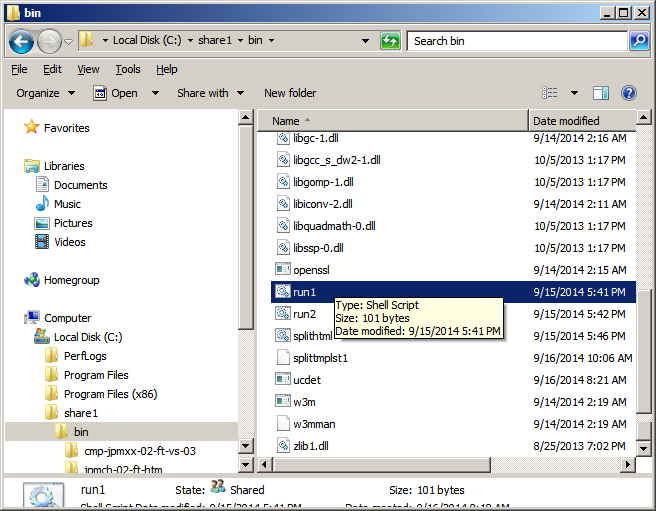
\includegraphics[width=0.45\textwidth]{figures/click-run1.png}
  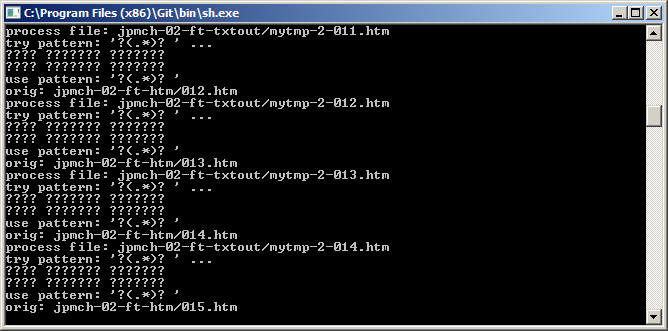
\includegraphics[width=0.45\textwidth]{figures/run1-screen.png}
  \caption{运行 \texttt{run1.sh} 时屏幕截图。}\label{fig:run1screen}
\end{figure}





\subsubsection{后续整理}

自动拆分后文件可能会存在些片段在一些小文件中,需要将无用的小文件删除,有用的要和其他分片文件合并(参见图 \ref{fig:deletesmall})。
手工对比确认是为了两个对比目录中各个文件的内容一一对应。一一对应的文件不一定需要文件名一样,而是其文件名在目录中排序后相对顺序一样,程序会顺序先后对比文件。


\begin{figure}[ht]\centering
  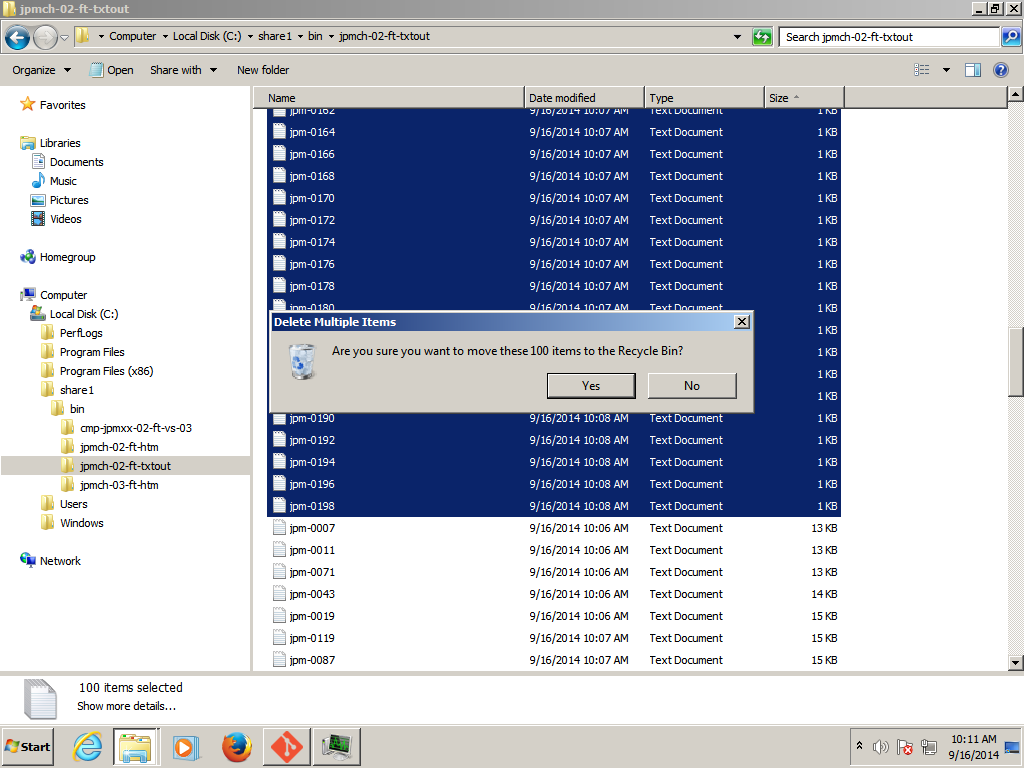
\includegraphics[width=0.85\textwidth]{figures/delete-trash.png}
  \caption{删除小文件。这些文件在 Windows 上显示为1K, 但实际大小只有300字节左右。检查时,按字节大小排序文件(如图中通过按``Size''那列的头就可排序),可以在打开检查文件内容后,选择这些小文件删除。}\label{fig:deletesmall}
\end{figure}


\clearpage

\subsection{对比章节} \label{chap:compcoll}

这个是软件的核心功能。在前面对数据做预处理后,现在就可以开始对比文档了。

\subsubsection{原理}

脚本 \texttt{compcolldir.sh} 是通过调用核心程序 \texttt{compcoll} 实现文件对比功能。


\subsubsection{参数和测试脚本}

脚本 \texttt{compcolldir.sh} 接受三个基本参数:旧文本的输入目录名、新文本的输入目录名、以及对比输出结果文件目录名。

使用参数 \texttt{-h} 或者 \texttt{--help} 可以列出所有支持的参数:
\begin{lstlisting}[language=bash]
./compcolldir.sh -h

Compare the files in two folders
Written by yhfu, 2014-09

./compcolldir.sh [options] [<old dir> [<new dir> [<out dir>]]] 

Options:
	--help|-h                     Print this message
	--prefix|-p <PREFIX>          Use the user's PREFIX as the prefix of data name (default: )
	--mergesame|-m                Merge adjacent changes
	--outreturn|-r <old|new|all>  Output the 'return'
	--singleout|-s                Use single output file

Examples:
  ./compcolldir.sh -h        # Print this message.
\end{lstlisting}


\textbf{输出文件名的前缀}

如果您还要设置输出文件名的前缀,可以使用参数 \texttt{-p} 来设置,如
\begin{lstlisting}[language=bash]
./compcolldir.sh -p jpm-
\end{lstlisting}

则让输出文件名像 ``\texttt{jpm-0000000000000000012.htm}'' 那样的格式,而不是缺省的 ``\texttt{0000000000000000012.htm}''。


你可以在测试脚本 \texttt{run2.sh} 中设置相关参数满足自己的需求。


\textbf{设置换行}

换行可以设置成 ``遵从旧文本''、``遵从新文本''、和 ``同时遵从旧文本或新文本'';
缺省是``遵从新文本''。
这个可以通过在命令行添加参数 \texttt{-r} 来实现:
\begin{lstlisting}[language=bash]
# 遵从旧文本
./compcolldir.sh -r old

# 遵从新文本
./compcolldir.sh -r new

# 同时遵从旧文本或新文本
./compcolldir.sh -r all
\end{lstlisting}


\textbf{设置显示变化的方式是合并修改还是分开}

各个字符的变化(插入、删除等)
可以设置成 ``分开各个字符的修改''、和 ``合并修改'';
缺省是``分开各个字符的修改''。
如果需要合并修改,可以通过在命令行添加参数 \texttt{-m} 来实现:
\begin{lstlisting}[language=bash]
./compcolldir.sh -m
\end{lstlisting}





\subsubsection{后续}

这个是最后一步了,直接打开输出目录中的 HTML 文件即可。
如果要修改显示风格,参见章节 \ref{chap:softsetup}。

对于一个典型的文本对比,其耗费内存大概是 700 MB 左右,见图 \ref{fig:compcollmem}。


\begin{figure}[ht]\centering
  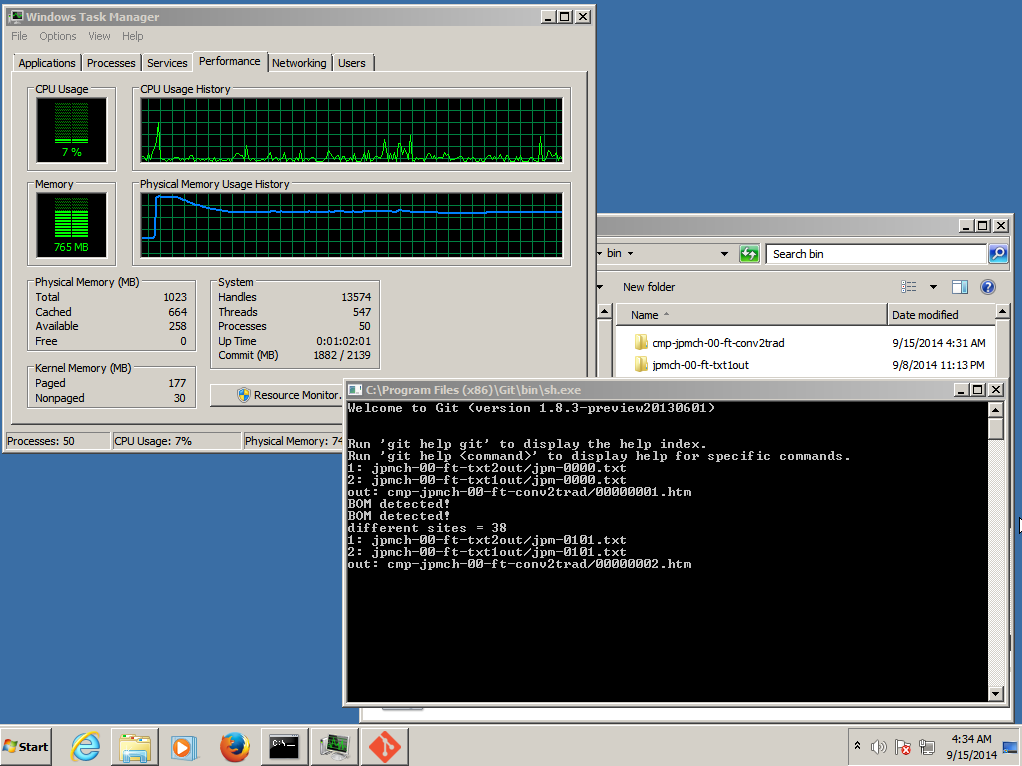
\includegraphics[width=0.45\textwidth]{figures/run4.png}
  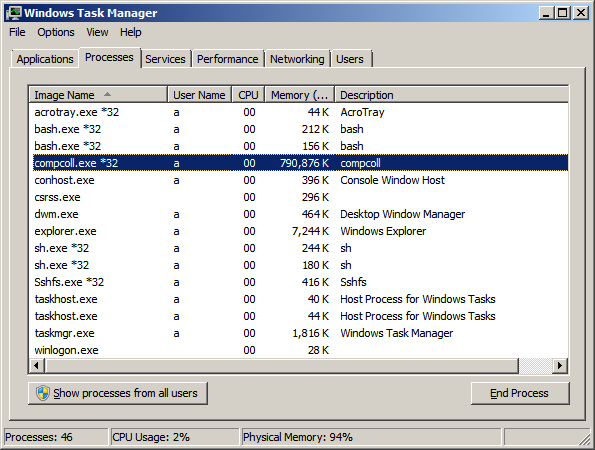
\includegraphics[width=0.45\textwidth]{figures/run-mem.png}
  \caption{运行 \texttt{compcolldir.sh} 时内存消耗情况。}\label{fig:compcollmem}
\end{figure}



\clearpage
\subsection{软件微调} \label{chap:softsetup}
可以针对自己的喜好,对软件做一些微调。

注意以下修改脚本文件时,建议不要用 Windows 自带的编辑器,因为可能会破坏脚本内容。
推荐使用开源软件 \href{http://code.google.com/p/madedit-pv/}{MadEdit},
下载安装请参考章节 \ref{chap:madeditinstall}。

\subsubsection{输出单个对比文件}
软件缺省是输出对比每个单独的章节为一个单独的文件,如果需要输出所有章节的对比内容到一个文件,如 \texttt{results.htm},
则可以
在调用脚本文件 \texttt{compcolldir.sh} 时,添加参数 \texttt{--singleout | -s}:
\begin{lstlisting}[language=bash]
compcolldir.sh -s
\end{lstlisting}

完成存盘后,重新运行对比脚本(如例子中的脚本文件 \texttt{run2.sh})。



\subsubsection{对比文字的颜色}

输出文件采用 HTML 格式,而且使用了 CSS,所以可以很方便地调整显示的风格。
一个方便调制对比文字风格的方法是使用和输出HTML文件放在一起的 CSS 文件 \texttt{compcollouter.css}。

如要将校对文字修改为绿色,可以编辑文件 \texttt{compcollouter.css} 成这样:
\footnote{你可以复制附带例子输出 HTML 文件中文件头中的 style 部分到这个文件中,这里的例子是基于那段配置的。}
\begin{lstlisting}[language=html]
  ins {
    color:green; font-weight: normal;
  }
  del,
  strike {
    color:purple;
    text-decoration: none;
    line-height: 1.4;
    background-image: -webkit-gradient(linear, left top, left bottom, from(transparent), color-stop(0.63em, transparent), color-stop(0.63em, #ff0000), color-stop(0.7em, #ff0000), color-stop(0.7em, transparent), to(transparent));
    background-image: -webkit-linear-gradient(top, transparent 0em, transparent 0.63em, #ff0000 0.63em, #ff0000 0.7em, transparent 0.7em, transparent 1.4em);
    background-image: -o-linear-gradient(top, transparent 0em, transparent 0.63em, #ff0000 0.63em, #ff0000 0.7em, transparent 0.7em, transparent 1.4em);
    background-image: linear-gradient(to bottom, transparent 0em, transparent 0.63em, #ff0000 0.63em, #ff0000 0.7em, transparent 0.7em, transparent 1.4em);
    -webkit-background-size: 1.4em 1.4em;
    background-size: 1.4em 1.4em;
    background-repeat: repeat;
  }
\end{lstlisting}

修改后,刷新浏览器即可看到效果。


\section{总结}

\texttt{compcoll} 是一个优化了的文本对比软件,结合 \texttt{bash} 脚本技术,可以定制用户的文本处理流程。
本说明描述了软件原理以及用户可如何定制软件使之能适用于自己的项目。


\end{document}
\endinput
%%
%% End of file `example-fallback.tex'.
